\section{Experiments and results}\label{sec:experiments}

\subsection{Data}\label{sec:data}

The multi-parametric \ac{mri} data are acquired from a cohort of patients with higher-than-normal level of \ac{psa}.
The acquisition is performed using a 3T whole body \ac{mri} scanner (Siemens Magnetom Trio TIM, Erlangen, Germany) using sequences to obtain \ac{t2w}-\ac{mri}, \ac{dce}-\ac{mri} and \ac{dw}-\ac{mri}.
Aside of the \ac{mri} examination, these patients also have underwent a guided-biopsy.
The dataset is composed of a total of 20 patients of which 18 patients have biopsy proven \ac{cap} and 2 patients are ``healthy'' with negative biopsies.
Therefore, 13 patients have a \ac{cap} in the \ac{pz}, 3 patients have \ac{cap} in the \ac{cg}, 2 patients have invasive \ac{cap} in both \ac{pz} and \ac{cg} and finally 2 patients are considered as ``healthy''.
An experienced radiologist has segmented the prostate organ --- on \ac{t2w}- and \ac{dce}-\ac{mri} --- as well as the prostate zones (i.e., \ac{pz} and \ac{cg}) and \ac{cap} on the \ac{t2w}-\ac{mri}.

The \ac{dce}-\ac{mri} sequence consists in a kinetic study composed of 40 samples over time with a time resolution of \SI{6.5}{\second}.
These \ac{dce}-\ac{mri} sequences are resampled using the spatial information of the \ac{t2w} \ac{mri} sequence with dimensions of $448 \times 360 \times 64$ and voxel spacing of $0.68 \times 0.68 \times 1.25 $ mm\textsuperscript{3}.
A linear interpolation is used to compute missing data during the up-sampling.
The volumes of the \ac{dce}-\ac{mri} dynamic are rigidly registered, to remove any patient motion during the acquisition.
Furthermore, a non-rigid registration is performed between the \ac{t2w}- and \ac{dce}-\ac{mri} in order to propagate the prostate zones and \ac{cap} ground-truths.
The resampling is implemented in C++ using the Insight Segmentation and Registration Toolkit~\citep{ibanez2005itk}.

\subsection{Results}

\begin{table}
  \caption{\acs*{auc} of the individual features for each method.}
  \centering
  \begin{tabular}{l c c c c}
    \toprule
    \textbf{Features} & \multicolumn{2}{c}{Un-normalized data} & \multicolumn{2}{c}{Normalized data} \\
    & \acs*{rf} & \acs*{nb} & \acs*{rf} & \acs*{nb} \\
    \midrule
    \textbf{Brix model} & & & & \\
    \quad $A$         & 0.54 & 0.62 & 0.58 & 0.67 \\
    \quad $k_{el}$    & 0.55 & 0.52 & 0.54 & 0.61 \\
    \quad $k_{ep}$    & 0.51 & 0.52 & 0.51 & 0.58 \\
    \textbf{Hoffmann model} & & & & \\
    \quad $A$         & 0.52 & 0.50 & 0.51 & 0.56 \\
    \quad $k_{el}$    & 0.55 & 0.53 & 0.54 & 0.64 \\
    \quad $k_{ep}$    & 0.55 & 0.50 & 0.53 & 0.66 \\
    \textbf{Tofts model with population \ac{aif}} & & & & \\
    \quad $K_{trans}$ & 0.56 & 0.62 & 0.56 & 0.65 \\
    \quad $v_{e}$     & 0.51 & 0.50 & 0.50 & 0.52 \\
    \quad $v_{p}$     & 0.53 & 0.63 & 0.55 & 0.53 \\
    \textbf{Tofts model with patient \ac{aif}} & & & & \\
    \quad $K_{trans}$ & 0.57 & 0.66 & 0.56 & 0.65 \\
    \quad $v_{e}$     & 0.49 & 0.50 & 0.51 & 0.52 \\
    \quad $v_{p}$     & 0.53 & 0.37 & 0.57 & 0.65 \\
    \textbf{\ac{pun} model} & & & & \\
    \quad $a_0$       & 0.52 & 0.53 & 0.53 & 0.51  \\
    \quad $r$         & 0.53 & 0.59 & 0.55 & 0.55 \\
    \quad $\beta$     & 0.55 & 0.56 & 0.53 & 0.44 \\
    \textbf{Semi-quantitative analysis} & & & & \\
    \quad wash-in     & 0.59 & 0.64 & 0.55 & 0.51 \\
    \quad wash-out    & 0.52 & 0.50 & 0.56 & 0.66 \\
    \quad IAUC        & 0.51 & 0.61 & 0.52 & 0.64 \\
    \quad $\tau$      & 0.57 & 0.57 & 0.56 & 0.61 \\
    \quad $S_M - S_0$ & 0.56 & 0.63 & 0.53 & 0.64 \\
    \bottomrule
  \end{tabular}
  \label{tab:resfeats}
\end{table}

\begin{figure}
  \centering
  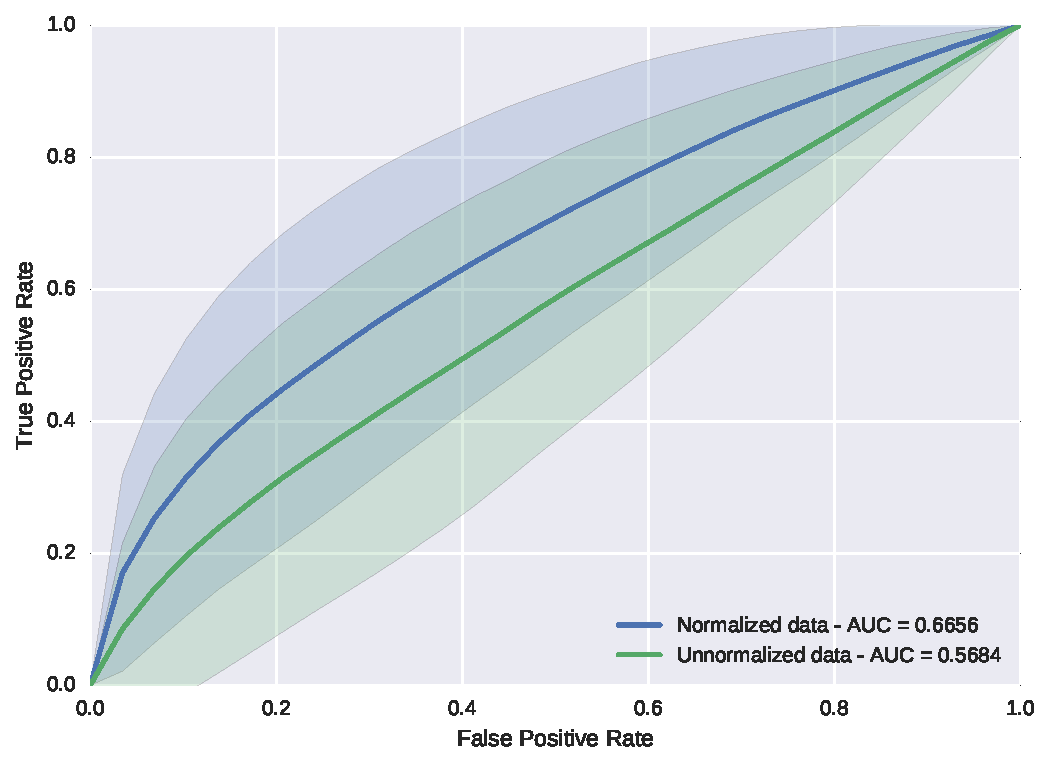
\includegraphics[width=0.7\linewidth]{03_experiments/figures/rf.pdf}
  \caption{\acs*{roc} analysis using a \acs*{rf} classifier using the \ac{dce} signal with and without normalization.}
  \label{fig:rfunorm}
\end{figure}

\begin{figure}
  \centering
  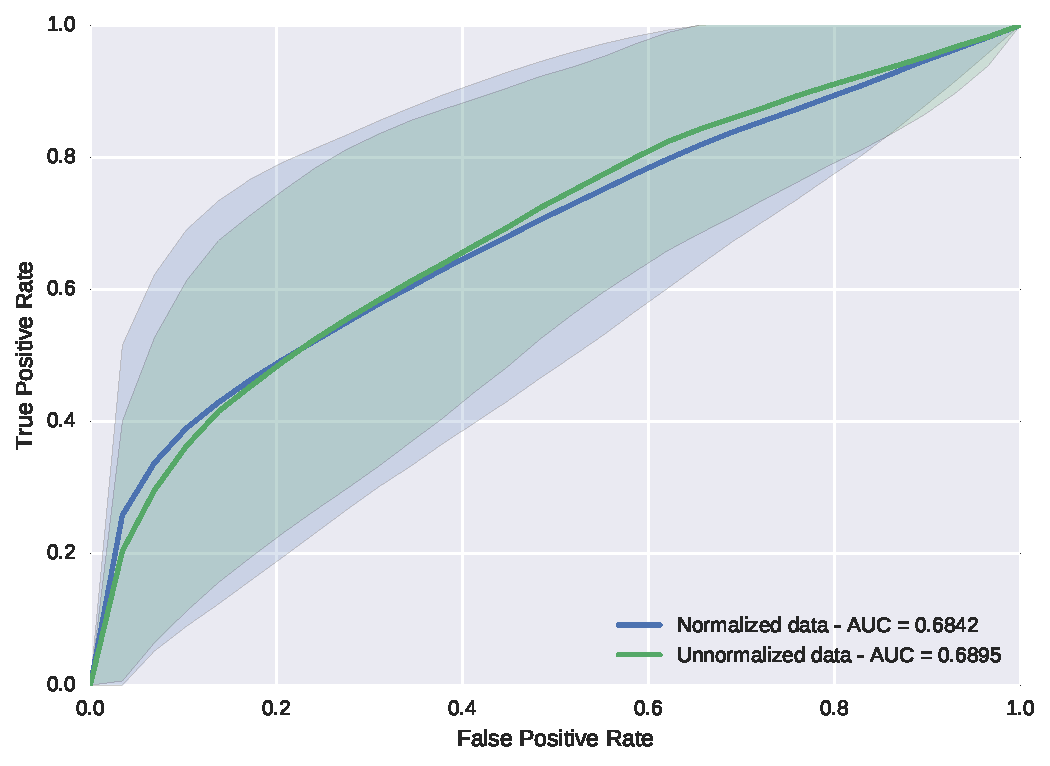
\includegraphics[width=0.7\linewidth]{03_experiments/figures/nb.pdf}
  \caption{\acs*{roc} analysis using a \acs*{nb} classifier using the \ac{dce} signal with and without normalization.}
  \label{fig:rfunorm}
\end{figure}

\begin{figure}
  \centering
  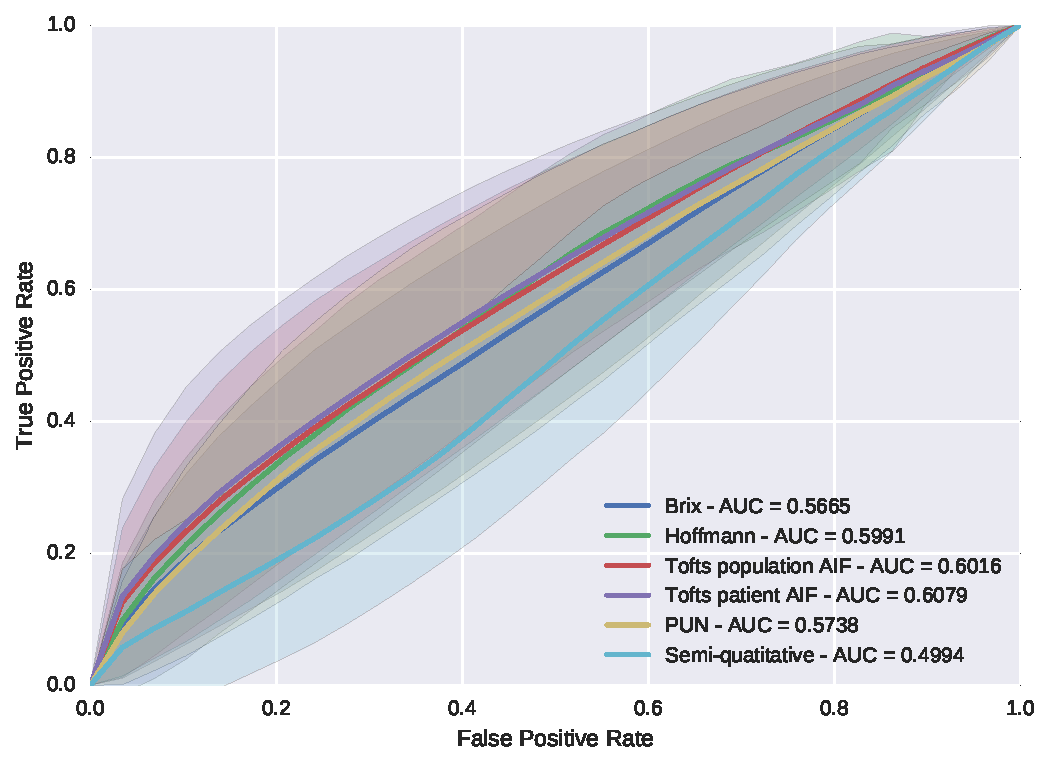
\includegraphics[width=0.7\linewidth]{03_experiments/figures/unormalized/rf.pdf}
  \caption{\acs*{roc} analysis using a \acs*{rf} classifier for the different quantification methods without data normalization.}
  \label{fig:rfunorm}
\end{figure}

\begin{figure}
  \centering
  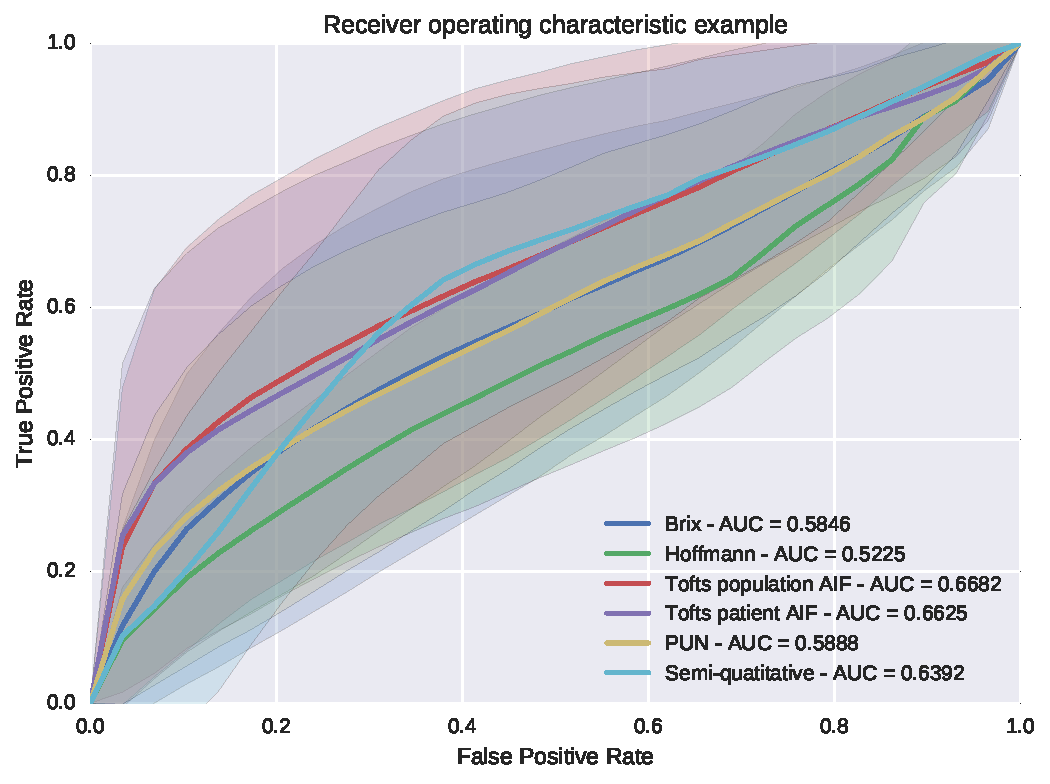
\includegraphics[width=0.7\linewidth]{03_experiments/figures/unormalized/nb.pdf}
  \caption{\acs*{roc} analysis using a \acs*{nb} classifier for the different quantification methods without data normalization.}
  \label{fig:rfunorm}
\end{figure}

\begin{figure}
  \centering
  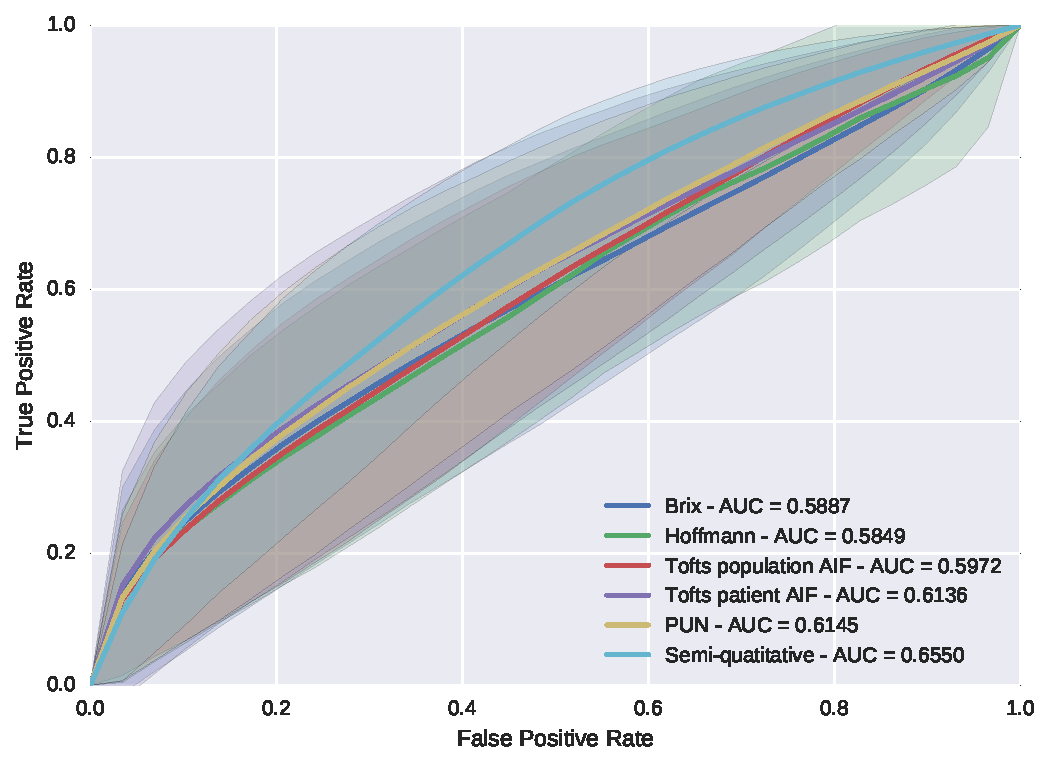
\includegraphics[width=0.7\linewidth]{03_experiments/figures/normalized/rf.pdf}
  \caption{\acs*{roc} analysis using a \acs*{rf} classifier for the different quantification methods with data normalization.}
  \label{fig:rfunorm}
\end{figure}

\begin{figure}
  \centering
  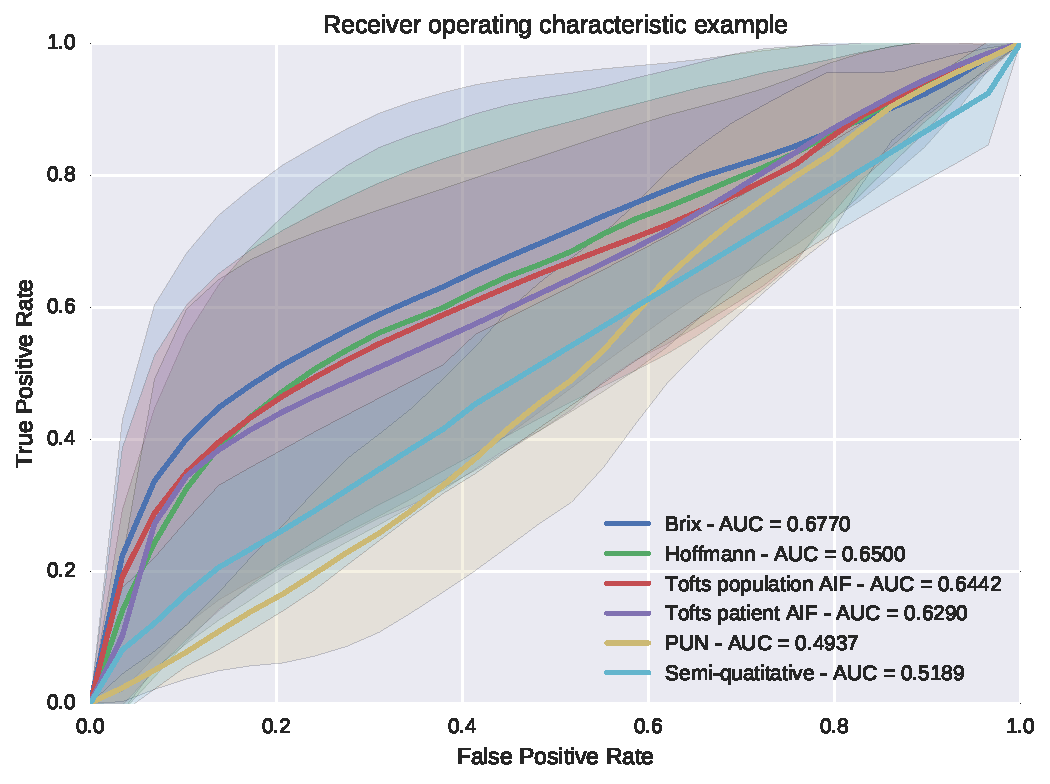
\includegraphics[width=0.7\linewidth]{03_experiments/figures/normalized/nb.pdf}
  \caption{\acs*{roc} analysis using a \acs*{nb} classifier for the different quantification methods with data normalization.}
  \label{fig:rfunorm}
\end{figure}

%%% Local Variables: 
%%% mode: latex
%%% TeX-master: "../main"
%%% End: 
